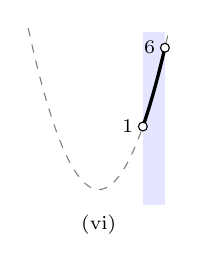
\begin{tikzpicture}[x=2.8mm,y=2mm]
\fill[blue!10] (4,-4) rectangle (5,7);
\ax{-1.6}{5.6}{-4}{7}
\draw[dashed,gray,domain=-1.2:5.2,samples=80] plot (\x,{(\x-2)^2-3});
\draw[very thick,domain=4:5,samples=80] plot (\x,{(\x-2)^2-3});
\draw[fill=white] (4,1) circle (1.6pt);
\node[left] at (4,1){\scriptsize 1};
\draw[fill=white] (5,6) circle (1.6pt);
\node[left] at (5,6){\scriptsize 6};
\node[below] at (current bounding box.south){\scriptsize (vi)};
\end{tikzpicture}